\section{Analysis}

As a group our task was to create a software product to work on. Our aim was to find a common interest, so we would all have the same level of enthusiasm about the project. A few hours of brainstorming have led us to decide on a fitness application. 
The product is an online coaching application. The target audience can be divided into two categories: coaches and trainees. The application would function similar to LinkedIn where the coaches would have to create a portfolio in order to attract trainees or customers. They can list their degree, training routine, specialties and photos. The trainees would decide based on this portfolio page to contact the coaches.
This product is different from other applications as it offers an opportunity to receive 1 on 1 training for a below market price. Moreover, the coaches would have time to focus on their clients closely as they would be able to take on only a few customers at the same time.
We created this product to people who want to improve their health by exercising while staying in their budget. The target audience is wide as the coaches can have various background and take on trainees with different goals and needs. Starting from people who want to gain weight or lose weight all the way to people who want to improve their mobility classifies as our target audience because the coaches who sign up provide the application with variety.
The opportunity of the product is the cost efficiency. Personal training has become an expensive service. The goal of this application is to have affordable coaches. While personal trainers only check in with you when you are training together, the coaches in our application can be available for your need at any time of the day and help you out with nutritional questions as well.

\subsection{User Journey Maps}
\label{sec:UserJourneyMaps}
In order to make sure that our application is easy to use we had to create user journey maps. When we created the app, we realized that our user can be divided into two groups, coaches and trainees. The two types of user are closely connected and when one of them does an action it will have an effect on the other user. The user journey maps are presented in the picture below.

\begin{figure}[H]
    \centering
    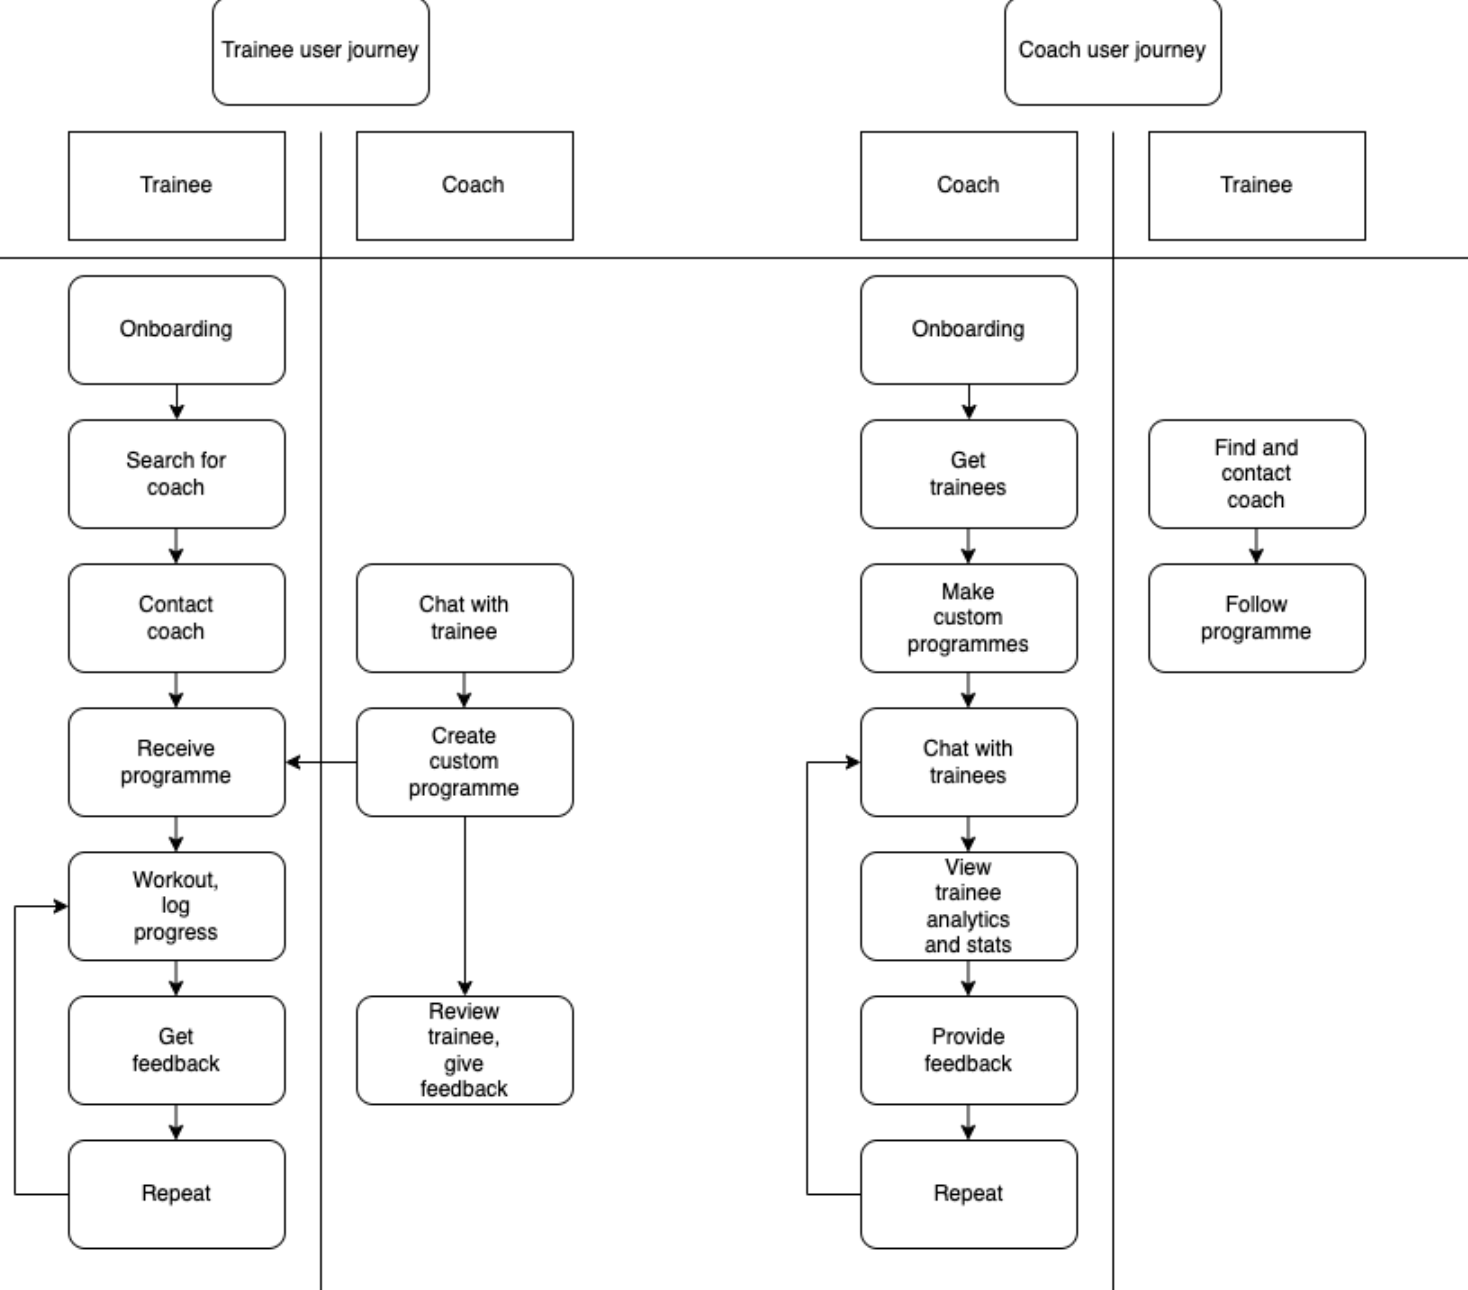
\includegraphics[width=1\textwidth]{Resources/UserJourneyMaps.png}
    \caption{User Journey Maps}
    \label{fig:UserJourneyMaps}
  \end{figure}


\subsection{Personas}
We had to create personas to make sure people with different goals and backgrounds could benefit from using our application. Diversity was our main goal while coming up with the personas. They were created using the software called Miro where each persona has their own brief description, skills, main goals, personality, interest, gains and pains listed. We have created 5 personas in total. 

\begin{figure}[H]
    \centering
    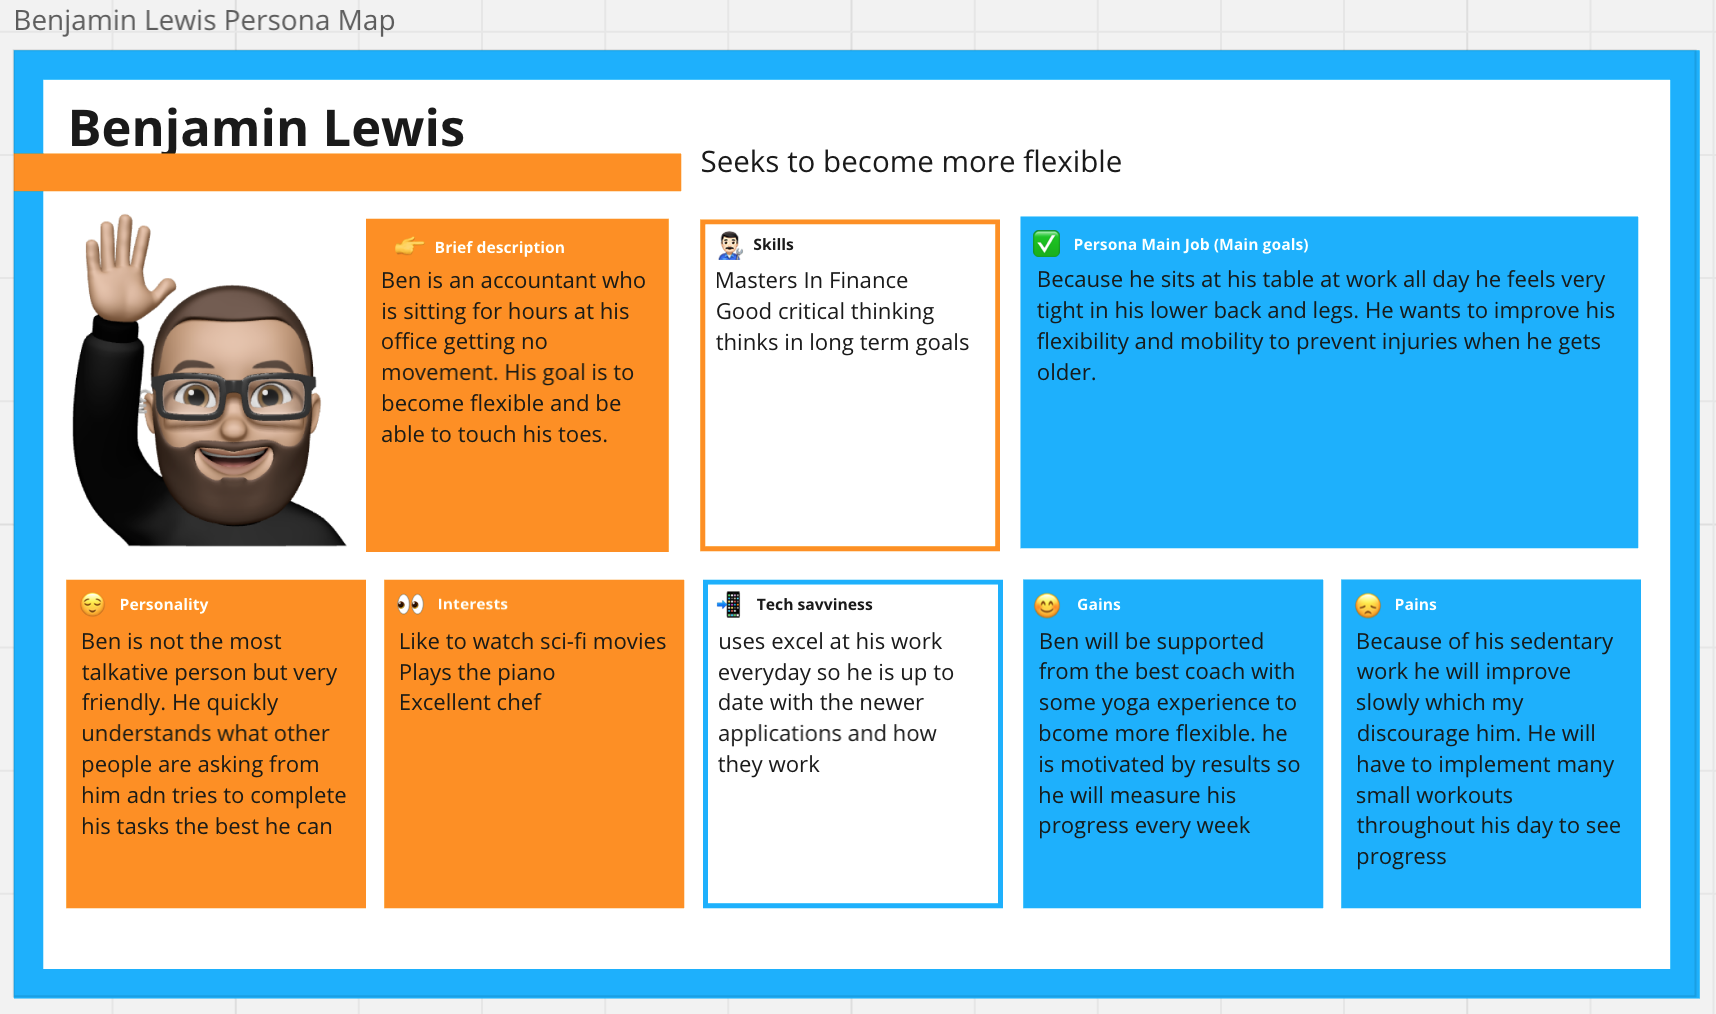
\includegraphics[width=1\textwidth]{Resources/BenjaminLewis.png}
    \caption{Benjamin Lewis}
    \label{fig:BenjaminLewis}
  \end{figure}
  \begin{figure}[H]
    \centering
    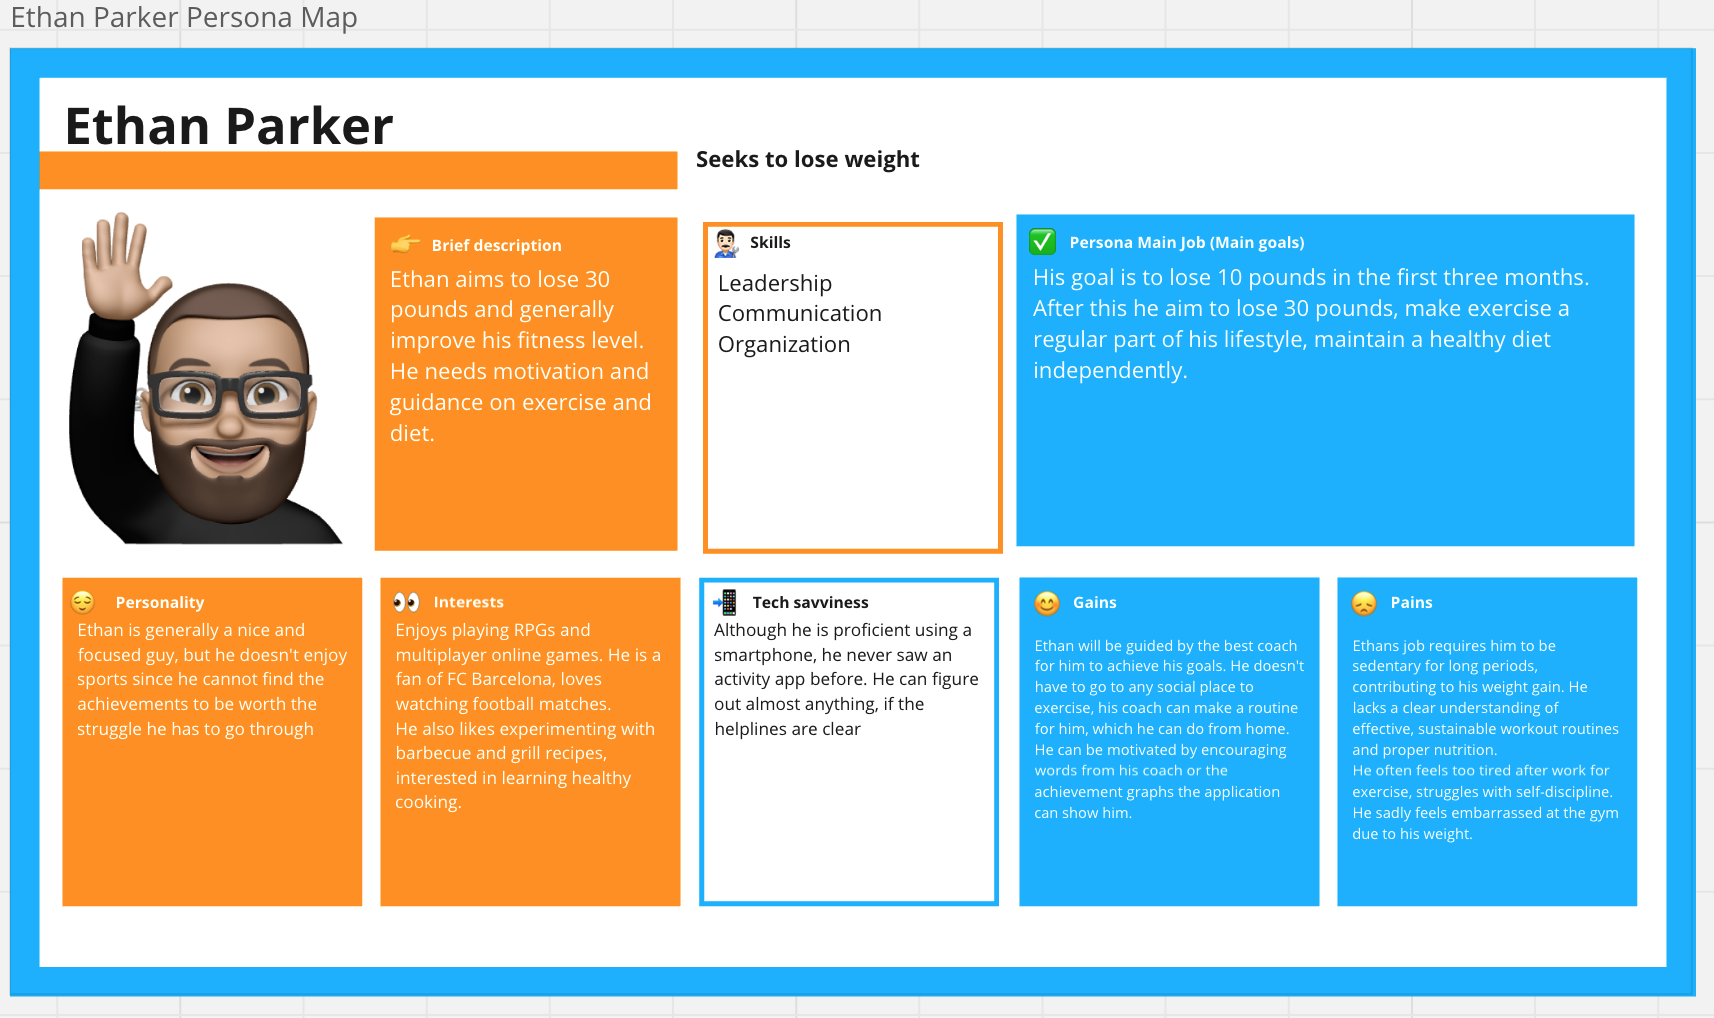
\includegraphics[width=1\textwidth]{Resources/EthanParker.png}
    \caption{Ethan Parker}
    \label{fig:EthanParker}
  \end{figure}
  \begin{figure}[H]
    \centering
    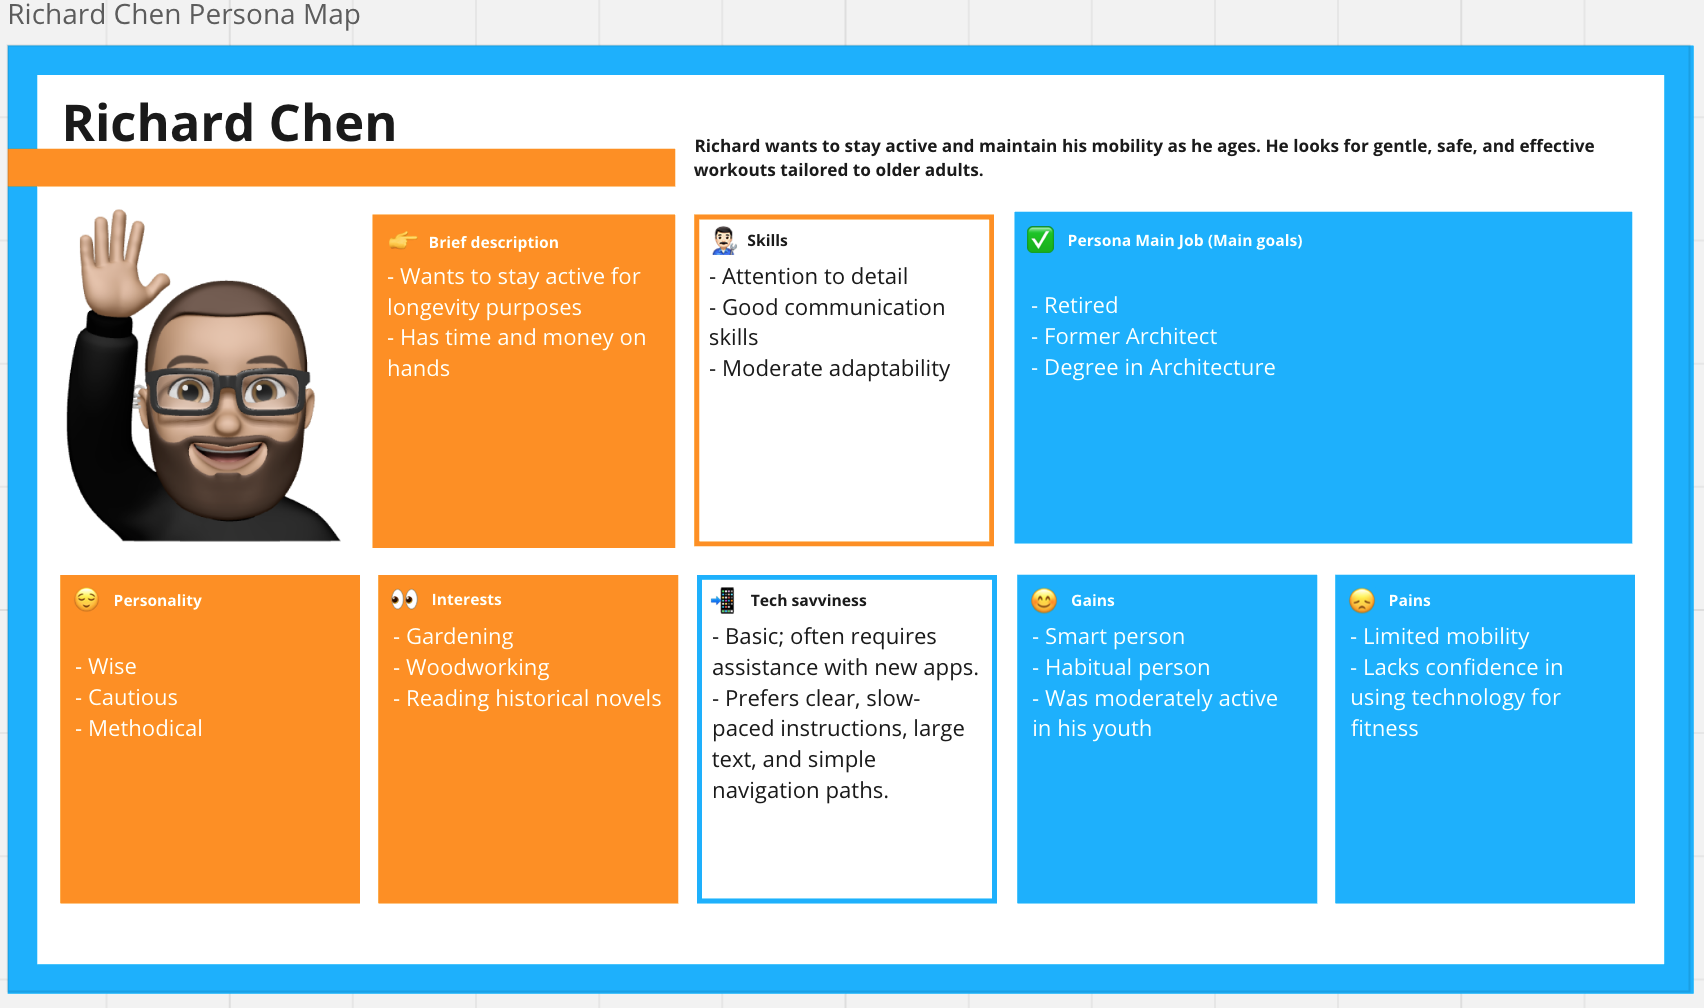
\includegraphics[width=1\textwidth]{Resources/RichardChen.png}
    \caption{Richard Chen}
    \label{fig:RichardChen}
  \end{figure}
  \begin{figure}[H]
    \centering
    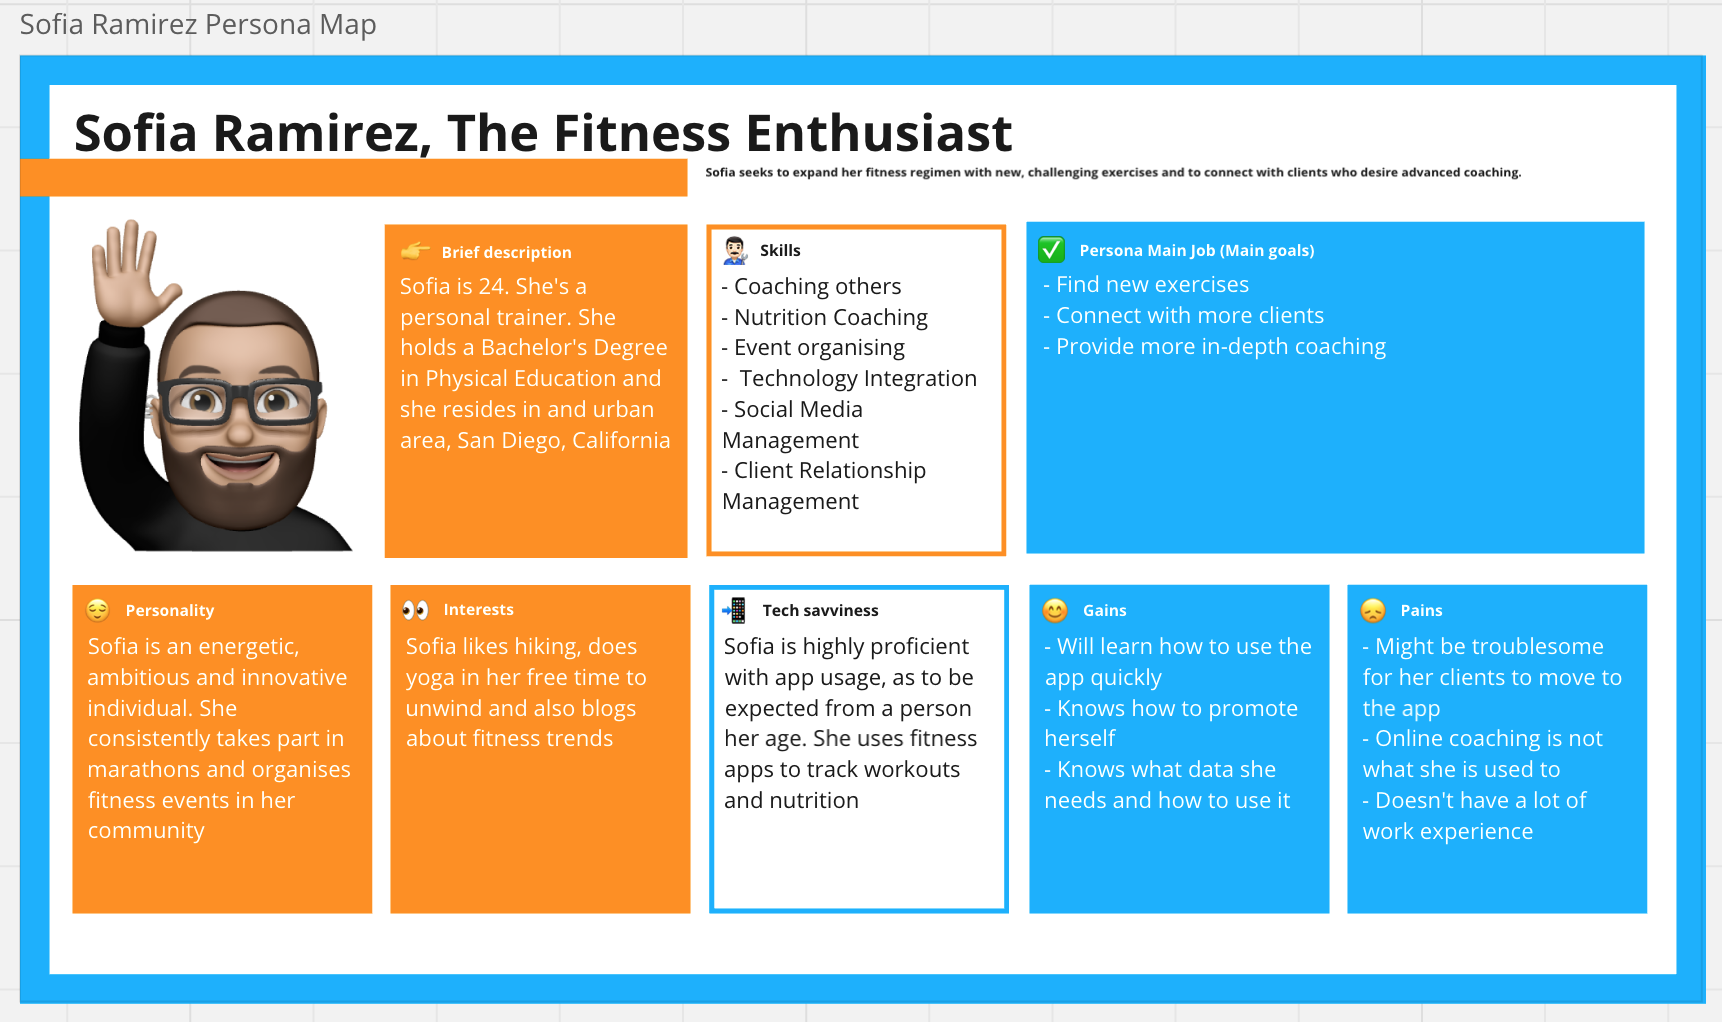
\includegraphics[width=1\textwidth]{Resources/SofiaRamirez.png}
    \caption{Sofia Ramirez}
    \label{fig:SofiaRamirez}
  \end{figure}
  \begin{figure}[H]
    \centering
    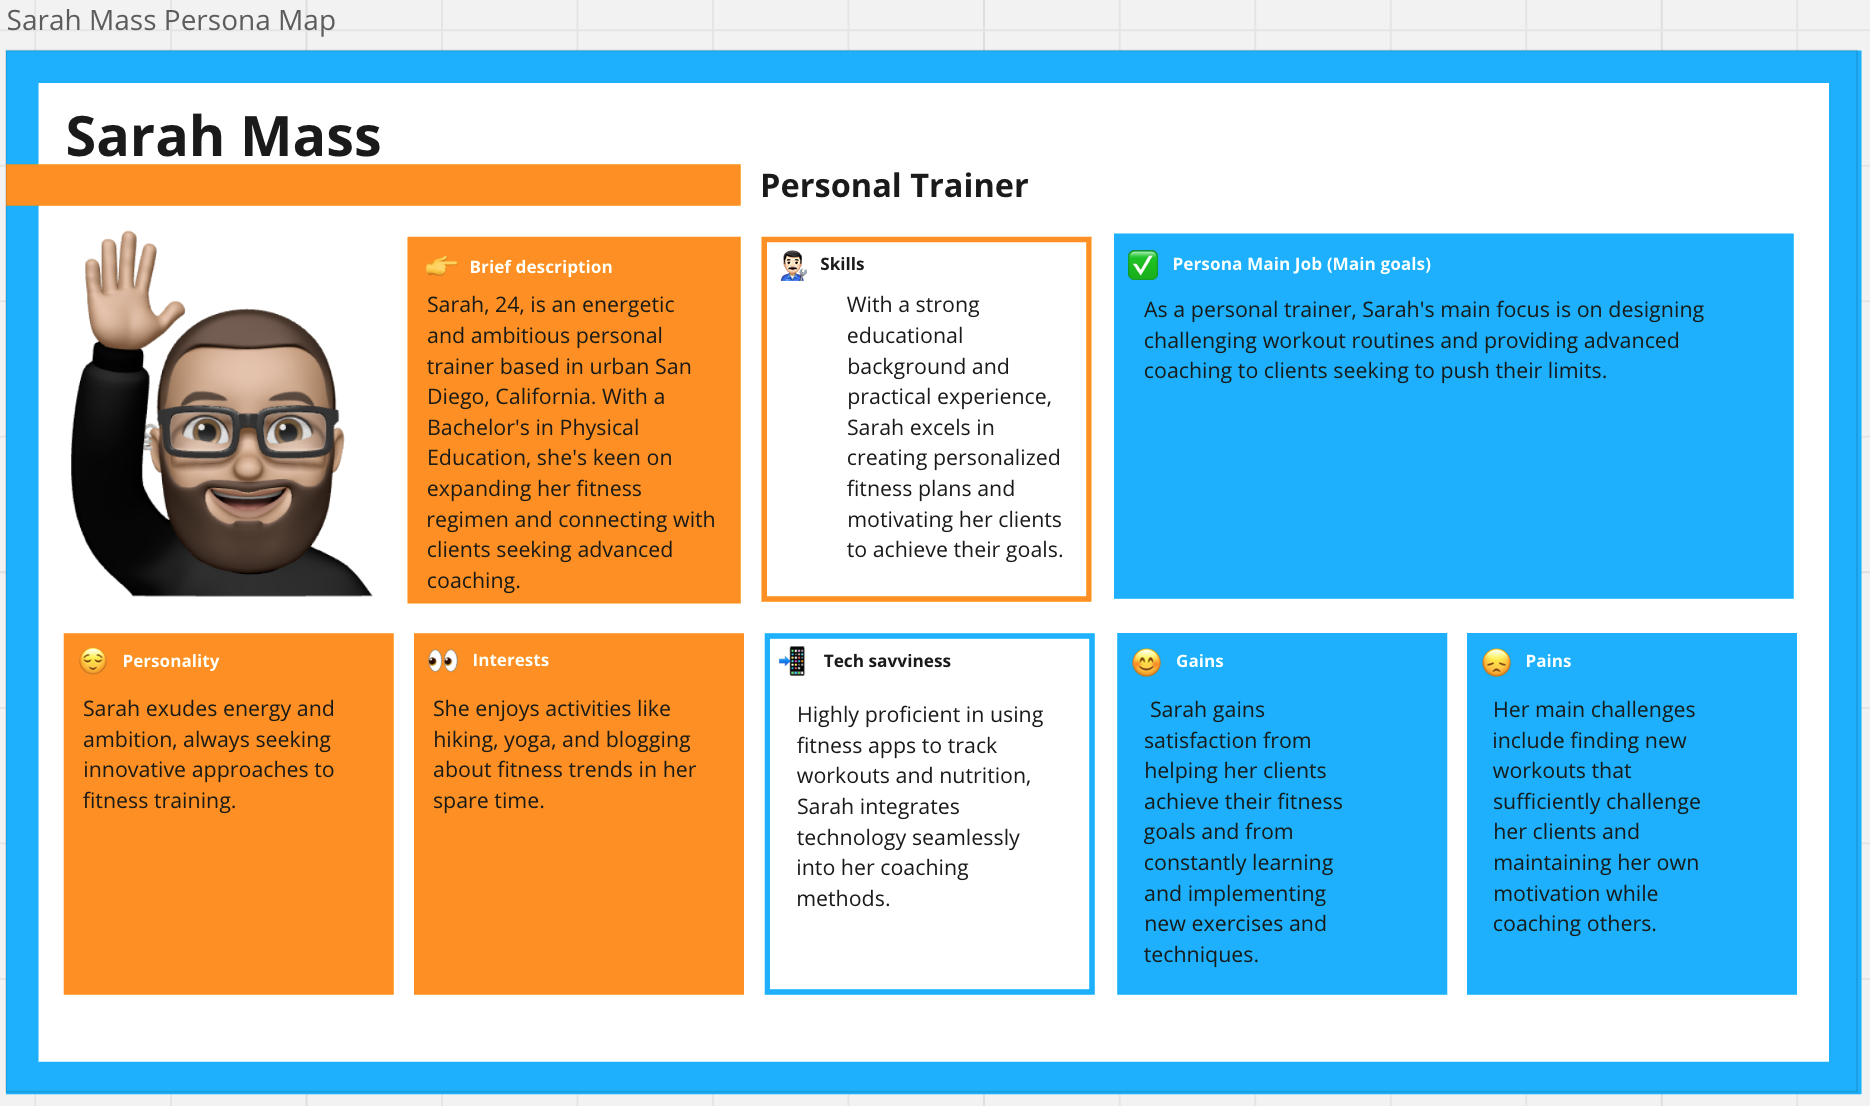
\includegraphics[width=1\textwidth]{Resources/SarahMass.png}
    \caption{Sarah Mass}
    \label{fig:SarahMass}
  \end{figure}

\subsection{Functional and non-functional requirements}
\label{sec:Requirements}
Functional requirements define the specific behaviours of a system. These requirements describe what the system should do in order to meet the user’s needs. Our application includes user authentication. There is a separate one for coaches and trainees but the system behind it is the same. In the application we have to include a payment processor as the coaches will likely provide subscription-based coaching. Through this system we will enable users to place, track and cancel orders. When creating a profile, we need to store the personal information in a database which can be updated by the user in the setting part of the application. In the application the trainees can search for preferred coaches therefore, the system allows users to search for coaches by various criteria, such as name, category and price range.
Non-functional requirements specify the quality attributes of a system. These requirements describe how the system performs certain functions such as usability, performance, reliability and security. The system should be user-friendly, allowing new users to find what they require in the app without extensive explanation. The system should also be able to handle several simultaneous users without performance issues while being available most of the time, even during software updates. The application has to be well encrypted to protect user data. 
\clearpage